
\section{Generación de números aleatorios} % Sections are added in order to organize your presentation into discrete blocks, all sections and subsections are automatically output to the table of contents as an overview of the talk but NOT output in the presentation as separate slides

%------------------------------------------------

\begin{frame}
	\frametitle{Distribución Uniforme}
	
	    \begin{columns}
		
		% Columna de la izquierda
		\begin{column}{0.5\textwidth} % Ajusta la proporción según necesites
			\begin{figure}
				\centering
				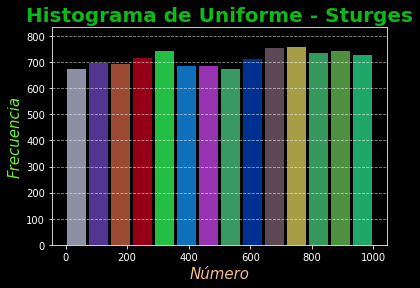
\includegraphics[width=\textwidth]{hist_uniform_Sturges} % Asegúrate de cambiar la ruta a la ubicación de tu imagen
				\caption{Histograma de distribución uniforme.}
			\end{figure}
		\end{column}
		
		% Columna de la derecha
		\begin{column}{0.5\textwidth} % Ajusta la proporción según necesites
			\begin{itemize}
				\item Se generó un archivo de \textit{10000} números aleatorios uniformemente distribuidos. 
				\item Se almacenan como \texttt{randomsUnifome.txt}
			\end{itemize}
		\end{column}
	\end{columns}
\end{frame}

%------------------------------------------------

